\subsection{变力沿直线所作的功}
\paragraph{}
如果物体在作直线运动的过程中有一个不变的力$F$作用在这个物体上,且这力的方向与物体运动的方向一致,那么在物体移动了距离$s$时,力$F$对物体所作的功为

\begin{equation}
  W = F \bigcdot s.
\end{equation}

\paragraph{}
如果物体在运动过程中所受到的力是变化的,这就会遇到变力对物体作功的问题。下面通过具体例子说明如何计算变力所作的功。

\begin{figure}[H]
\centering
  % 电荷做工
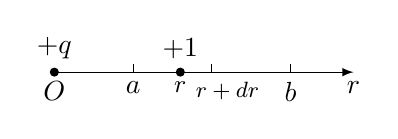
\begin{tikzpicture}[scale=1]
  \draw[-latex] (0,0) -- (3.8,0);
  \node[below] at (3.8,0) {$r$};

  \node[below] at (0,0) {$O$};
  \draw[fill=black] (0,0) circle (0.05cm);
  \node[above] at (0,0.05) {$+q$};

  \draw (1,0) -- (1,0.1);
  \node[below] at (1,0) {$a$};

  \node[below] at (1.6,0) {\small $r$};
  \node[above] at (1.6,0.05) {$+1$};
  \draw[fill=black] (1.6,0) circle (0.05cm);

  \draw (2,0) -- (2,0.1);
  \node[below] at (2.2,0) {\footnotesize $r+dr$};

  \draw (3,0) -- (3,0.1);
  \node[below] at (3,0) {$b$};
\end{tikzpicture}

  \caption{电荷做功}
  \label{电荷做功}
\end{figure}

\paragraph{}
\textbf{例1\;}把一个带电荷量$+q$的点电荷放在$r$轴上坐标原点$O$处,它产生一个电场。这个电场对周围的电荷有作用力。由物理学知道,如果有一个单位正电荷放在这个电场中距离原点$O$为$r$的地方,那么电场对它的作用力的大小为
\begin{equation}
  F = k\frac{q}{r^2} \; (k\text{是常数}).
\end{equation}

见图\figureref{电荷做功},当这个单位正电荷在电场中从$r=a$处沿$r$轴移动到$r=b \, (a<b)$处时,计算电场力$F$对它所作的功。

\paragraph{}
\textbf{解\;}在上述移动过程中,电场对这单位正电荷的作用力是变的,取$r$为积分变量,它的变化区间为$[a,b]$。设$[r,r+dr]$为$[a,b]$上的任一小区间。当单位正电荷从$r$移动到$r+dr$时,电场力对它所作的功近似于$\displaystyle\frac{kq}{r^2}dr$,即功元素为
\begin{equation}
  dW = \frac{kq}{r^2}dr.
\end{equation}

\paragraph{}
于是所求的功为
\begin{equation}
  W = \int_a^b\frac{kq}{r^2}dr = kq\big[ -\frac{1}{r} \big]_a^b = kq\big( \frac{1}{a} - \frac{1}{b} \big).
\end{equation}

\paragraph{}
在计算静电场中某点的电位时,要考虑将单位正电荷从该点处($r=a$)移到无穷远处时,电场力所作的功$W$。此时,电场力对单位正电荷所作的功就是反常积分:

\begin{equation}
  W = \int_a^{+\infty}\frac{kq}{r^2}dr = \big[ -\frac{kq}{r} \big]_a^{+\infty} = \frac{kq}{a}.
\end{equation}

\subsection{水压力}
\paragraph{}
在水深为$h$处的压强为$p = \rho gh$,这里$\rho$是水的密度,$g$是重力加速度。如果有一面积为$A$的平板水平地放置在水深为$h$处,那么,平板一侧所受的水压力为

\begin{equation}
  P = p \bigcdot A.
\end{equation}

\paragraph{}
如果平板铅直放置在水中,那么,由于水深不同的点处压强$p$不相等,平板一侧所受的水压力就不能用上述方法计算。下面举例说明它的计算方法。

\paragraph{}
\textbf{例2\;}一个横着放着的圆柱形水桶,桶内盛有半桶水(图\linkref[横放着的圆柱水桶水压a]{(\ref{横放着的圆柱水桶水压} - a)})。设桶的底半径为$R$,水的密度为$\rho$,计算桶的一个端面上所受的压力。

\begin{figure}[h]
\centering
  %------- 第1行 -------
  \begin{subfigure}[t]{0.42\linewidth}
    \centering
      % 水压力例子(a)
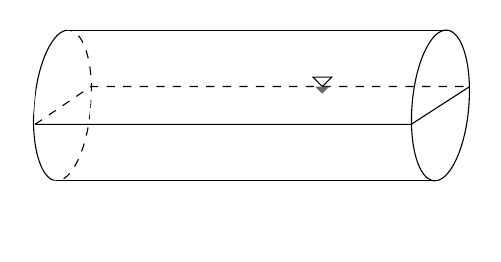
\begin{tikzpicture}[scale=0.6]
  % \draw [help lines] (-1,-3) grid (9,3);

  % 左椭圆
  \begin{scope}
    \clip[rotate=-5] (-0.6,-1.6) rectangle (0,1.6);
    \draw[rotate=-5] (0,0) ellipse [x radius=0.6cm,y radius=1.6cm];
  \end{scope}
  \begin{scope}
    \clip[rotate=-5] (0,-1.6) rectangle (0.6,1.6);
    \draw[dashed,rotate=-5] (0,0) ellipse [x radius=0.6cm,y radius=1.6cm];
  \end{scope}

  % 上下边框
  \draw (0.139,1.593) -- (8.139,1.593);
  \draw (-0.139,-1.593) -- (7.861,-1.593);

  % 水面
  \draw (-0.58,-0.4) -- (7.38,-0.4) -- (8.62,0.4);
  \draw[dashed] (-0.58,-0.4) -- (0.6,0.4) -- (8.62,0.4);

  \draw (5.5,0.4) -- (5.3,0.6) -- (5.7,0.6) -- (5.5,0.4);
  \path[fill=black!60] (5.5,0.25) -- (5.35,0.4) -- (5.65,0.4) -- (5.5,0.25);

  % 右椭圆
  \draw[rotate around={-5:(8,0)}] (8,0) ellipse [x radius=0.6cm,y radius=1.6cm];

  % 空白,提升高度,底部的 padding
  \draw[white] (0,-2.7) -- (0.01,-2.7);
\end{tikzpicture}

      \caption{}
      \label{横放着的圆柱水桶水压a}
  \end{subfigure}
  \begin{subfigure}[t]{0.42\linewidth}
    \centering
      % 水压力例子(b)
\begin{tikzpicture}[scale=0.6]
  \node[below] at (2.6,0) {$y$};
  \draw[-latex] (-2.6,0) -- (2.6,0);
  \node[left] at (0,-2.6) {$x$};
  \draw[-latex] (0,2.6) -- (0,-2.6);
  \draw (0,0) circle (1.6cm);

  \draw (1.2,0) -- (1,0.2) -- (1.4,0.2) -- (1.2,0);
  \path[fill=black!60] (1.2,-0.15) -- (1.05,0) -- (1.35,0) -- (1.2,-0.15);

  \node[above left] at (0,0) {$O$};
  \node[below right] at (1.5,0.05) {\small $R$};

  \node[above right] at (-0.05,-0.6) {$x$};

  \draw[pattern=north east lines] (-1.45,-0.6) -- (1.45,-0.6) -- (1.45,-0.9) -- (-1.45,-0.9) -- (-1.45,-0.6);
  \node[below right] at (-0.05,-0.9) {\footnotesize $x+dx$};
\end{tikzpicture}

      \caption{}
      \label{横放着的圆柱水桶水压b}
  \end{subfigure}

  \caption{横放着的圆柱水桶水压}
  \label{横放着的圆柱水桶水压}
\end{figure}

\paragraph{}
\textbf{解\;}桶的一个端面是圆片,所以现在要计算的是当水平面通过圆心时,铅直放置的一个半圆片的一侧所受到的水压力。

\paragraph{}
如图\linkref[横放着的圆柱水桶水压b]{(\ref{横放着的圆柱水桶水压} - b)},在这个圆片上取过圆心且铅直向下的直线为$x$轴,过圆心的水平线为$y$轴。对这个坐标系来讲,所讨论的半圆的方程为$x^2+y^2=R^2 \; (0\leq x\leq R)$。取$x$为积分变量,它的变化区间为$[0,R]$。设$[x,x+dx]$为$[0,R]$上的任一小区间,半圆片上相应于$[x,x+dx]$的窄条上各点处的压强近似于$\rho gx$,这窄条的面积近似于$\displaystyle 2\sqrt{R^2-x^2}dx$。因此,这窄条一侧所受水压力的近似值,即压力元素为

\begin{equation}
dP = 2\rho gx \sqrt{R^2-x^2}dx.
\end{equation}

于是所求压力为
\begin{align}
  P \;=&\; \int_0^R 2\rho gx \sqrt{R^2-x^2}dx = -\rho g\int_0^R(R^2-x^2)^{1/2}d(R^2-x^2) \\
  \;=&\; -\rho g\big[ \frac{2}{3}(R^2-x^2)^{3/2} \big]_0^R = \frac{2\rho g}{3}R^3.
\end{align}

\subsection{引力}
\paragraph{}
质量分别为$m_1, m_2$,相距为$r$的两质点间的引力的大小为
\begin{equation}
  F = G\frac{m_1m_2}{r^2},
\end{equation}
其中$G$为引力系数,引力的方向沿着两质点的连线方向。

\paragraph{}
如要计算一根细棒对一个质点的引力,那么由于细棒上各点与该质点的距离是变化的,且各点对该质点的引力的方向也是变化的,因此就不能用上述公式来计算。下面举例说明它的计算方法。

\paragraph{}
\textbf{例3\;}设有一长度为$l$、线密度为$\mu$的均匀细直棒,在其中垂线上距棒$a$单位处有一质量为$m$的质点$M$。试计算该棒对质点$M$的引力。

\begin{figure}[H]
\centering
  % 引力应用
\begin{tikzpicture}[scale=0.6]

  \node[left] at (0,5) {$y$};
  \draw[-latex] (0,-5) -- (0,5);
  \node[below] at (7,0) {$x$};
  \draw[-latex] (0,0) -- (7,0);

  % M
  \node[below right] at (4,0) {$M$};
  \draw[fill=black] (4,0) circle (0.08cm);
  \draw[-latex] (4,0) -- (0,2);

  % y
  \node[left] at (-0.15,2) {$y$};
  \draw (0,2) -- (-0.15,2);

  \node[left] at (-0.15,2.6) {$y+dy$};
  \draw (0,2.6) -- (-0.15,2.6);

  \node[below] at (2,0) {$a$};

  \draw[line width=0.05cm] (0,3.5) -- (0,-3.5);
  \node[left] at (0,3.5) {$\frac{l}{2}$};
  \node[left] at (0,-3.5) {$-\frac{l}{2}$};

  \node[above right] at (2,1) {$r$};

  % 原点
  \node [left] at (0,0) {$O$};
\end{tikzpicture}

  \caption{引力}
  \label{引力}
\end{figure}

\textbf{解\;}取坐标系如图\figureref{引力}所示,使棒位于$y$轴上,质点$M$位于$x$轴上,棒的中点为原点$O$。取$y$为积分变量,它的变化区间为$\big[-\frac{l}{2}, \frac{l}{2} \big]$。设$[y, y+dy]$为$\big[-\frac{l}{2}, \frac{l}{2} \big]$上任一小区间,把细直棒上相应于$[y,y+dy]$的一小段近似地看成质点,其质量为$\mu dy$,与$M$相距$\displaystyle r=\sqrt{a^2+y^2}$。因此可以按照两质点间的引力计算公式求出这小段细直棒对质点$M$的引力$\Delta F$的大小为

\begin{equation}
  \Delta F \approx G\frac{m\mu dy}{a^2+y^2},
\end{equation}

\paragraph{}
从而求出$\Delta F$在水平方向分力$\Delta F_x$的近似值,即细直棒对质点$M$的引力在水平方向分力$F_x$的元素为

\begin{equation}
  dF_x = -G\frac{am\mu dy}{(a^2+y^2)^{\frac{3}{2}}},
\end{equation}

于是得引力在水平方向分力为
\begin{align}
  F_x \;=&\; - \int_{-\frac{l}{2}}^{\frac{l}{2}} \frac{Gam\mu}{(a^2+y^2)^{\frac{3}{2}}} dy \\
  \;=&\; -\frac{2Gm\mu l}{a} \bigcdot \frac{1}{\sqrt{4a^2+l^2}}.
\end{align}
由对称性知,引力在铅直方向分力为$F_y=0$.

\paragraph{}
当细直棒的长度$l$很大时,可视$l$趋于无穷。此时,引力的大小为$\displaystyle \frac{2Gm\mu}{a}$,方向与细棒垂直且由$M$指向细棒。
